\subsection{Modelli Compartimentali}
In epidemiologia i modelli compartimentali sono una tecnica di modellezione 
generica che si predispone molto bene allo studio complessivo del comportamento
di una malattia infettiva \cite{wiki:Compartmental_models_in_epidemiology}. 
Questa tecnica di modellazione si applica anche ad altre branche della 
scienza, come ad esempio la finanza.

Questa tecnica di modellazione matematica basa il proprio funzionamento 
sull'assunzione che, data una popolazione di individui, questi vengano 
etichettati in maniera differente, in base allo stato di progressione 
della malattia che hanno, o non hanno, contratto. Così facendo si vanno a 
definire dei compartimenti ben separati che possono interagire tra loro, ma 
che rimangono comunque chiaramente distinti l'uni dagli altri.

Il modello che tutt'ora viene usato come riferimento e come base per 
lo studio e modellazione è il così detto modello 
Susceptible, Infectious, Recovered (SIR):

\begin{figure}[h]
    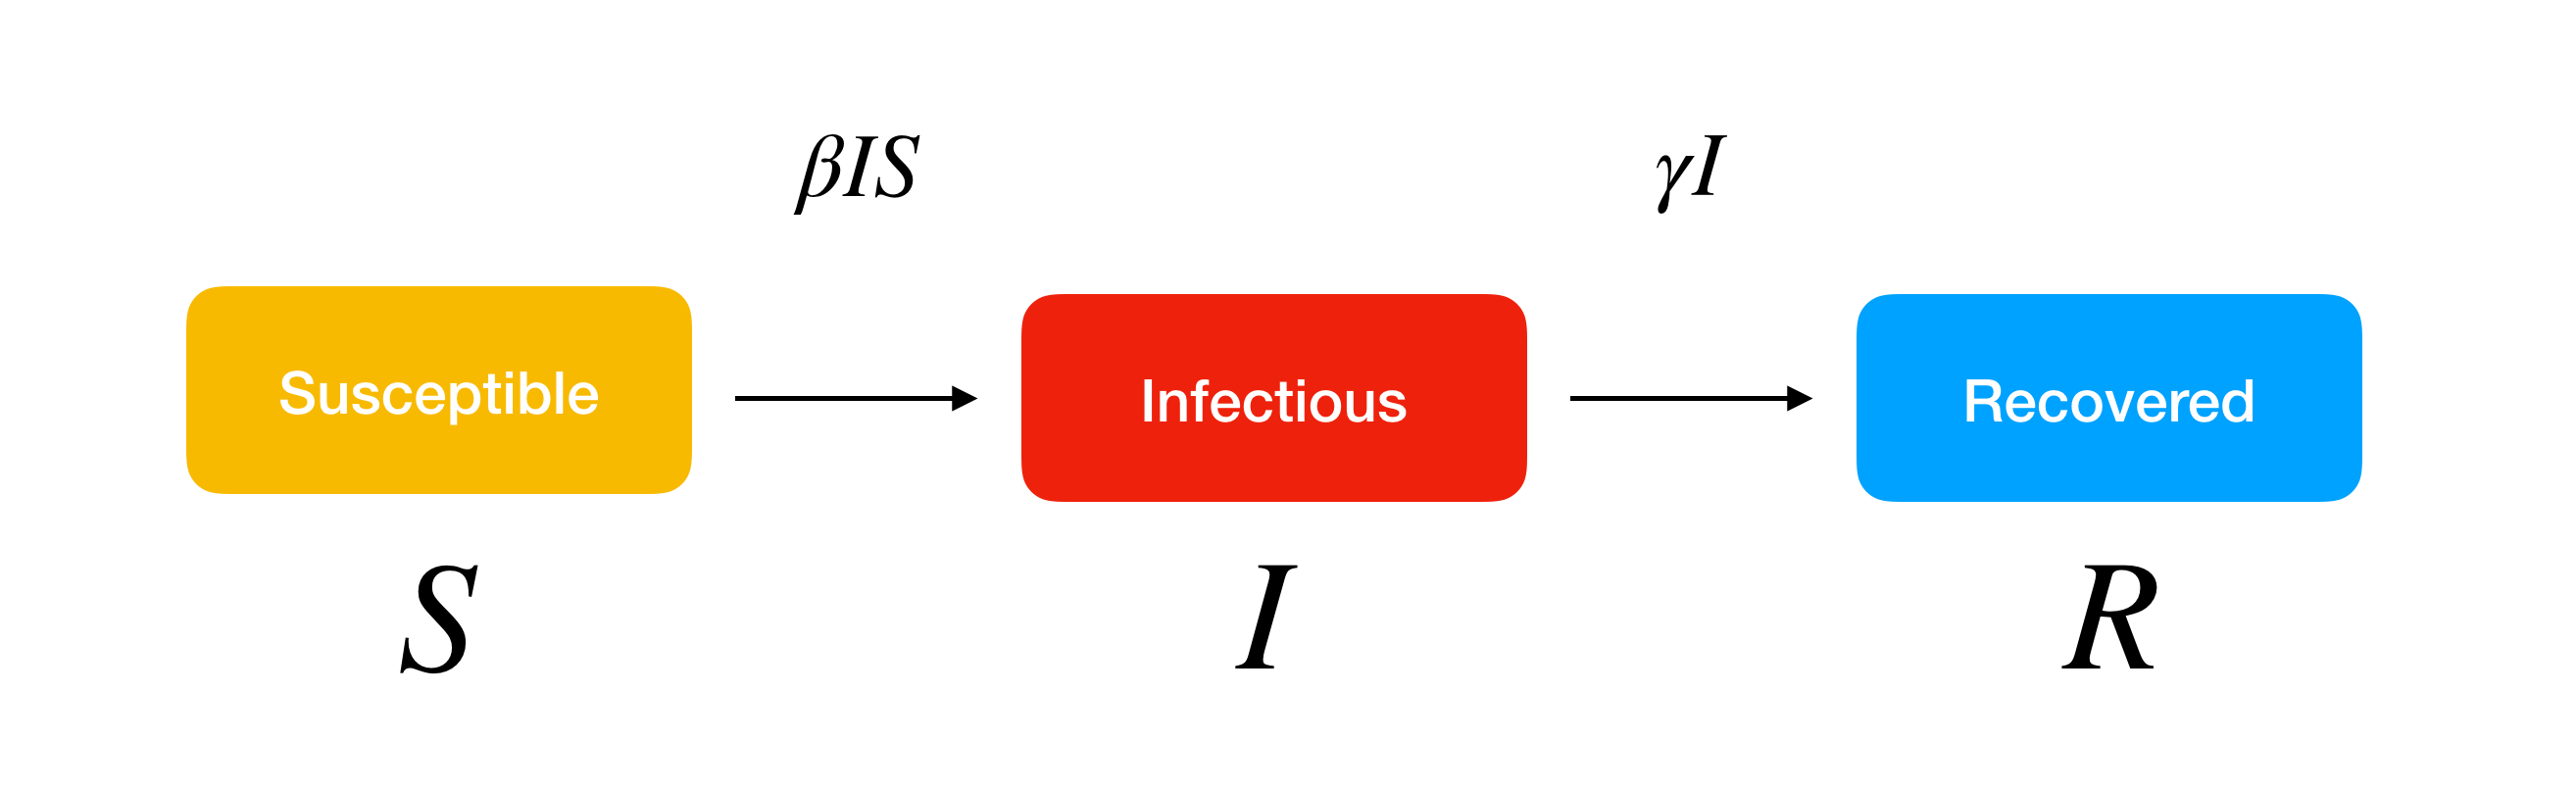
\includegraphics[width=\linewidth]{img/sir.png}
    \caption{Struttura modello SIR} 
    \label{fig:SIR_Structure}
\end{figure}

Questo modello è stato ideato all'inizio del 20esimo secolo, 
più precisamente nel 1917, da Kermack e McKendrick. Come introdotto questo modello
si basa sull'assunzione che all'interno di una popolazione durante 
il decorso di una malattia vi possano esistere solamente tre stadi in cui 
un individuo può essere inserito: 

\begin{itemize}
    \item Susceptible: Questo stadio rappresenta lo stato iniziale per la maggior parte
    degli individui all'interno di una popolazione. Rappresenta il numero di 
    persone che possono contrarre la malattia.
    \item Infectious: Questo stadio rappresenta tutti quegli individui che dallo 
    stato di Susceptible, dopo essere venuti in contatto con un individui infetto, 
    diventano a loro volta individui infetti.
    \item Recovered: Questo stadio rappresenta una duplice categoria, quella degli
    individui che alla fine del docorso della malattia sopravvivono ad essa, e 
    quelli che invece muoiono a causa di questa. Generalemente questo stato viene
    anche definito come Removed.
\end{itemize}

Da questa semplice idea poi si è andato a sviluppare un modello
matematico per descrivere come queste 3 categorie separate ma 
che si influenzano vicendevolmente, cambiano nel corso del tempo.
Questo approccio si basa sull'utilizzo di un sistema di Equazioni 
Ordinarie Differenziali (ODE) \cite{Brauer2008}. Una ODE è
un equazione differenziale, ovvero un equazione che lega 
una funzione incognita alle sue derivate, che coinvolge una 
funzione di una variabile e le sue derivate di ordine qualsiasi.
Questo oggetto viene utilizzato estensivamente in molti ambiti 
della scienza e in epidemiologia viene utilizzato per 
descrivere un sistema dinamico \cite{wiki:Equazione_differenziale_ordinaria}. 

\begin{figure}[h]
    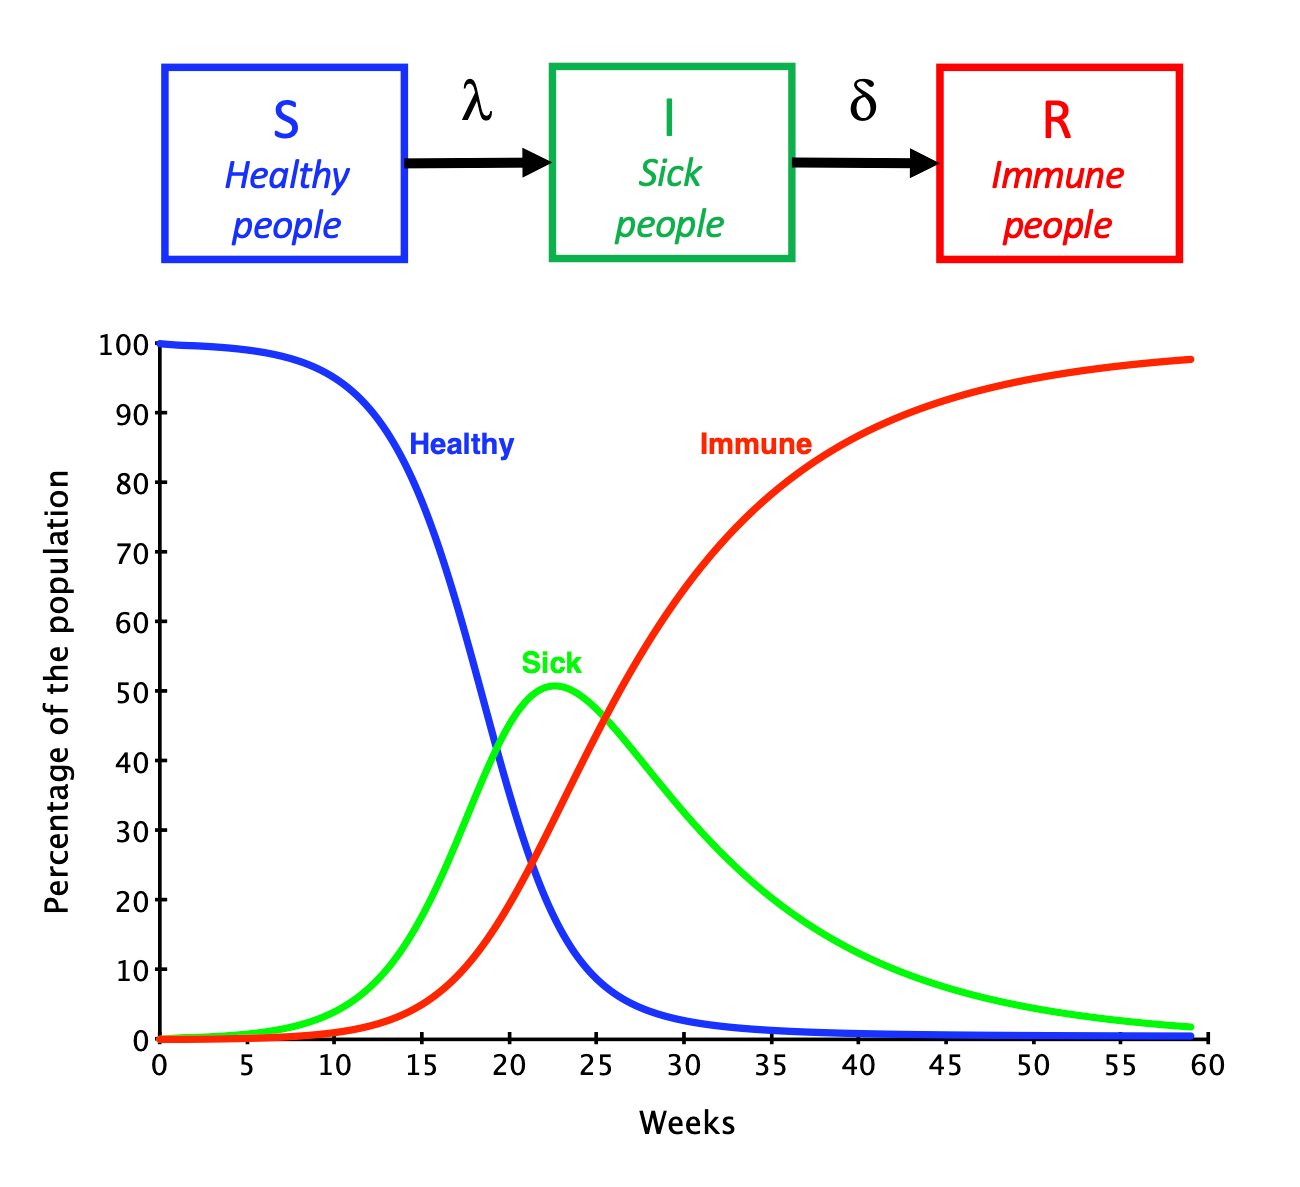
\includegraphics[width=\linewidth]{img/SIR-model.png}
    \caption{Visualizzazione grafico modello SIR} 
    \label{fig:SIR_model_graphic}
\end{figure}

Come succede per la maggior parte di tutte le equazioni 
differenziali, queste non possono essere solitamente 
risolte in maniera esatta, e per questo ci si limita a 
studiarne il comportamento qualitativo della soluzione 
senza essere capaci di ottenere una'espressione analitica.

Nell'ambito epidemiologico tuttavia non sempre l'utilizzo
di un sistema di ODE è preferito come metodo generale di 
modellazione di un sistema dinamico, in quanto il più 
delle volte questo sistema al suo interno utilizza un 
insieme di variabili rappresentanti processi stocastici, le quali 
è bene mantenere tali. A questo scopo vengono utilizzati i 
sistemi di Equazioni Differenziali Stocastiche (SDE) \cite{Allen2008}.

Queste equazioni si basano sulla teoria del moto Browniano 
il quale descrive il movimento randomico delle particelle 
sospese all'interno di un medium \cite{wiki:Brownian_motion}. 
In questo modo è possibile modellare in maniera più granulare
ad esempio la diffusione di un agente patogeno tramite il 
medium aereo, come può essere il COVID-19.

\subsubsection{Derivazioni del modello SIR}

Con il tempo questo il modello SIR è stato espanso 
per tenere in considerazione comportamenti
differenti sia della popolazione che delle malattie, 
andando a definire una moltitudine di modelli utili a 
differenti scopi. In epidemiologia il modello di
riferimento maggiormente utilizzato è il modello SEIR 
(Susceptible, Exposed, Infectious, Recovered)
con le sue varianti proprie di ogni approccio.

Questa tipologia di modello basa il proprio punto di forza
sull'osservazione che da quando un individuo viene 
infettato tramite un agente patogeno a quando quest'ultimo 
diventa infettivo, passa un periodo di latenza in cui 
l'individuo non può ne infettare ne essere infettato. 
Questo periodo viene anche conosciuto come periodo di 
incubazione \cite{wiki:Incubation_period}. Con questa 
conoscenza pregressa è possibile sviluppare modelli 
e policy che tenendo conto di questo comportamento lo 
sfruttino per arginare l'epidemia.

\begin{figure}[h]
    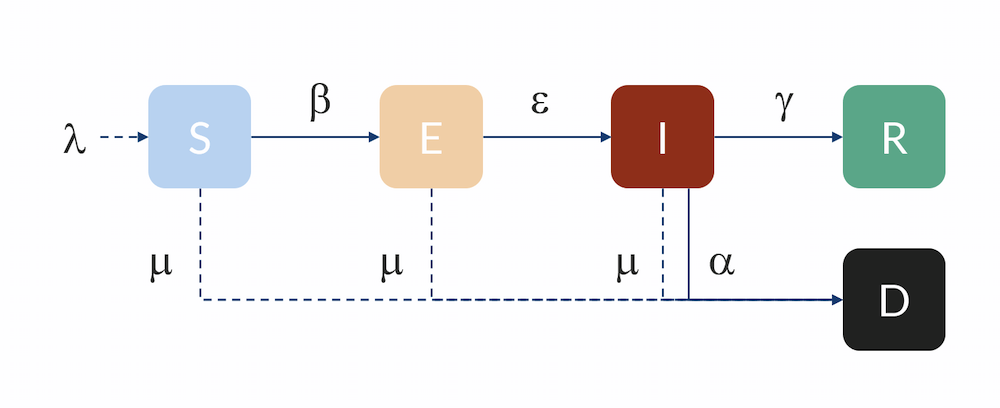
\includegraphics[width=\linewidth]{img/SEIR-compartmental-model-schematic.png}
    \caption{Modello schematico SEIR} 
    \label{fig:SEIR_model}
\end{figure}

Alcuni modelli definiscono i propri stati in maniera da considerare 
come stato interno al sistema anche l'agente patogeno, così da 
poter modellare e simulare l'andamento dell'infettività della pandemia 
in relazione alle contromisure prese, siano esse farmaceutiche o non.
Ne è un esempio il modello proposto da \cite{Mwalili2020} nel quale 
il modello viene proposto con l'idea di incorporare le misure di 
distanziamento sociale come variabili per misurare la loro efficacia
contro la recente pandemia da COVID-19.

\begin{figure}[h]
    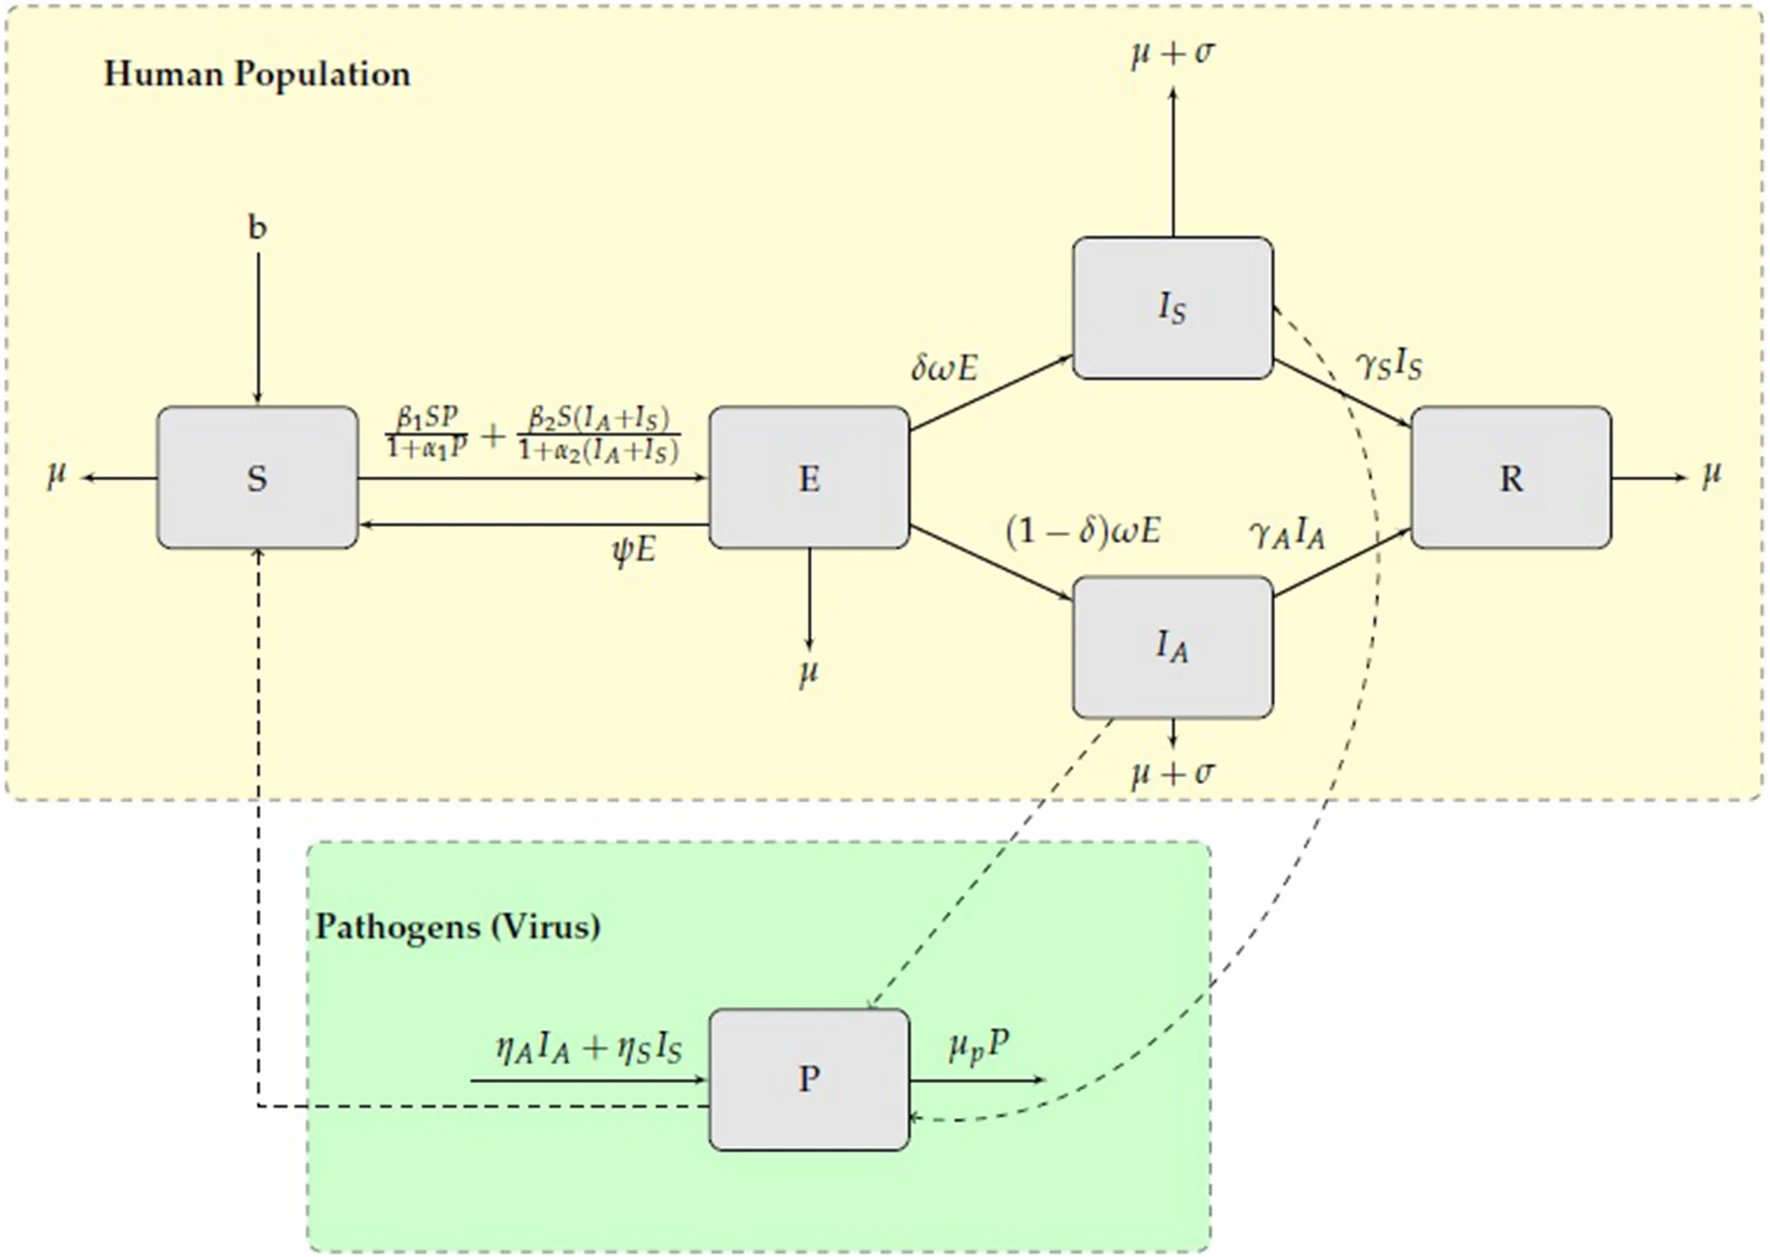
\includegraphics[width=\linewidth]{img/13104_2020_5192_Fig1_HTML.png}
    \caption{Esempio di modello SEIR preso dall'articolo \cite{Mwalili2020}}
    \label{fig:SEIR_model_social_distancing}
\end{figure}

Altri modelli, come quello proposto da \cite{ijerph17103535} mantengono 
la stessa filosofia, ovvero quella di analizzare l'efficacia delle misure 
di prevenzione non farmaceutiche sull'andamento di un epidemia, ma non
modellano esplicitamente l'agente patogeno come stato del modello, bensì
variando i paramentri di infettività e contagio, arrivano allo stesso 
risultato. Un'altra differenza tra i due approcci è quella della tipologia
di equazioni differenziali utilizzate, \cite{Mwalili2020} hanno utilizzato 
delle ODE mentre \cite{ijerph17103535} delle SDE.

\newpage

\begin{figure}[h]
    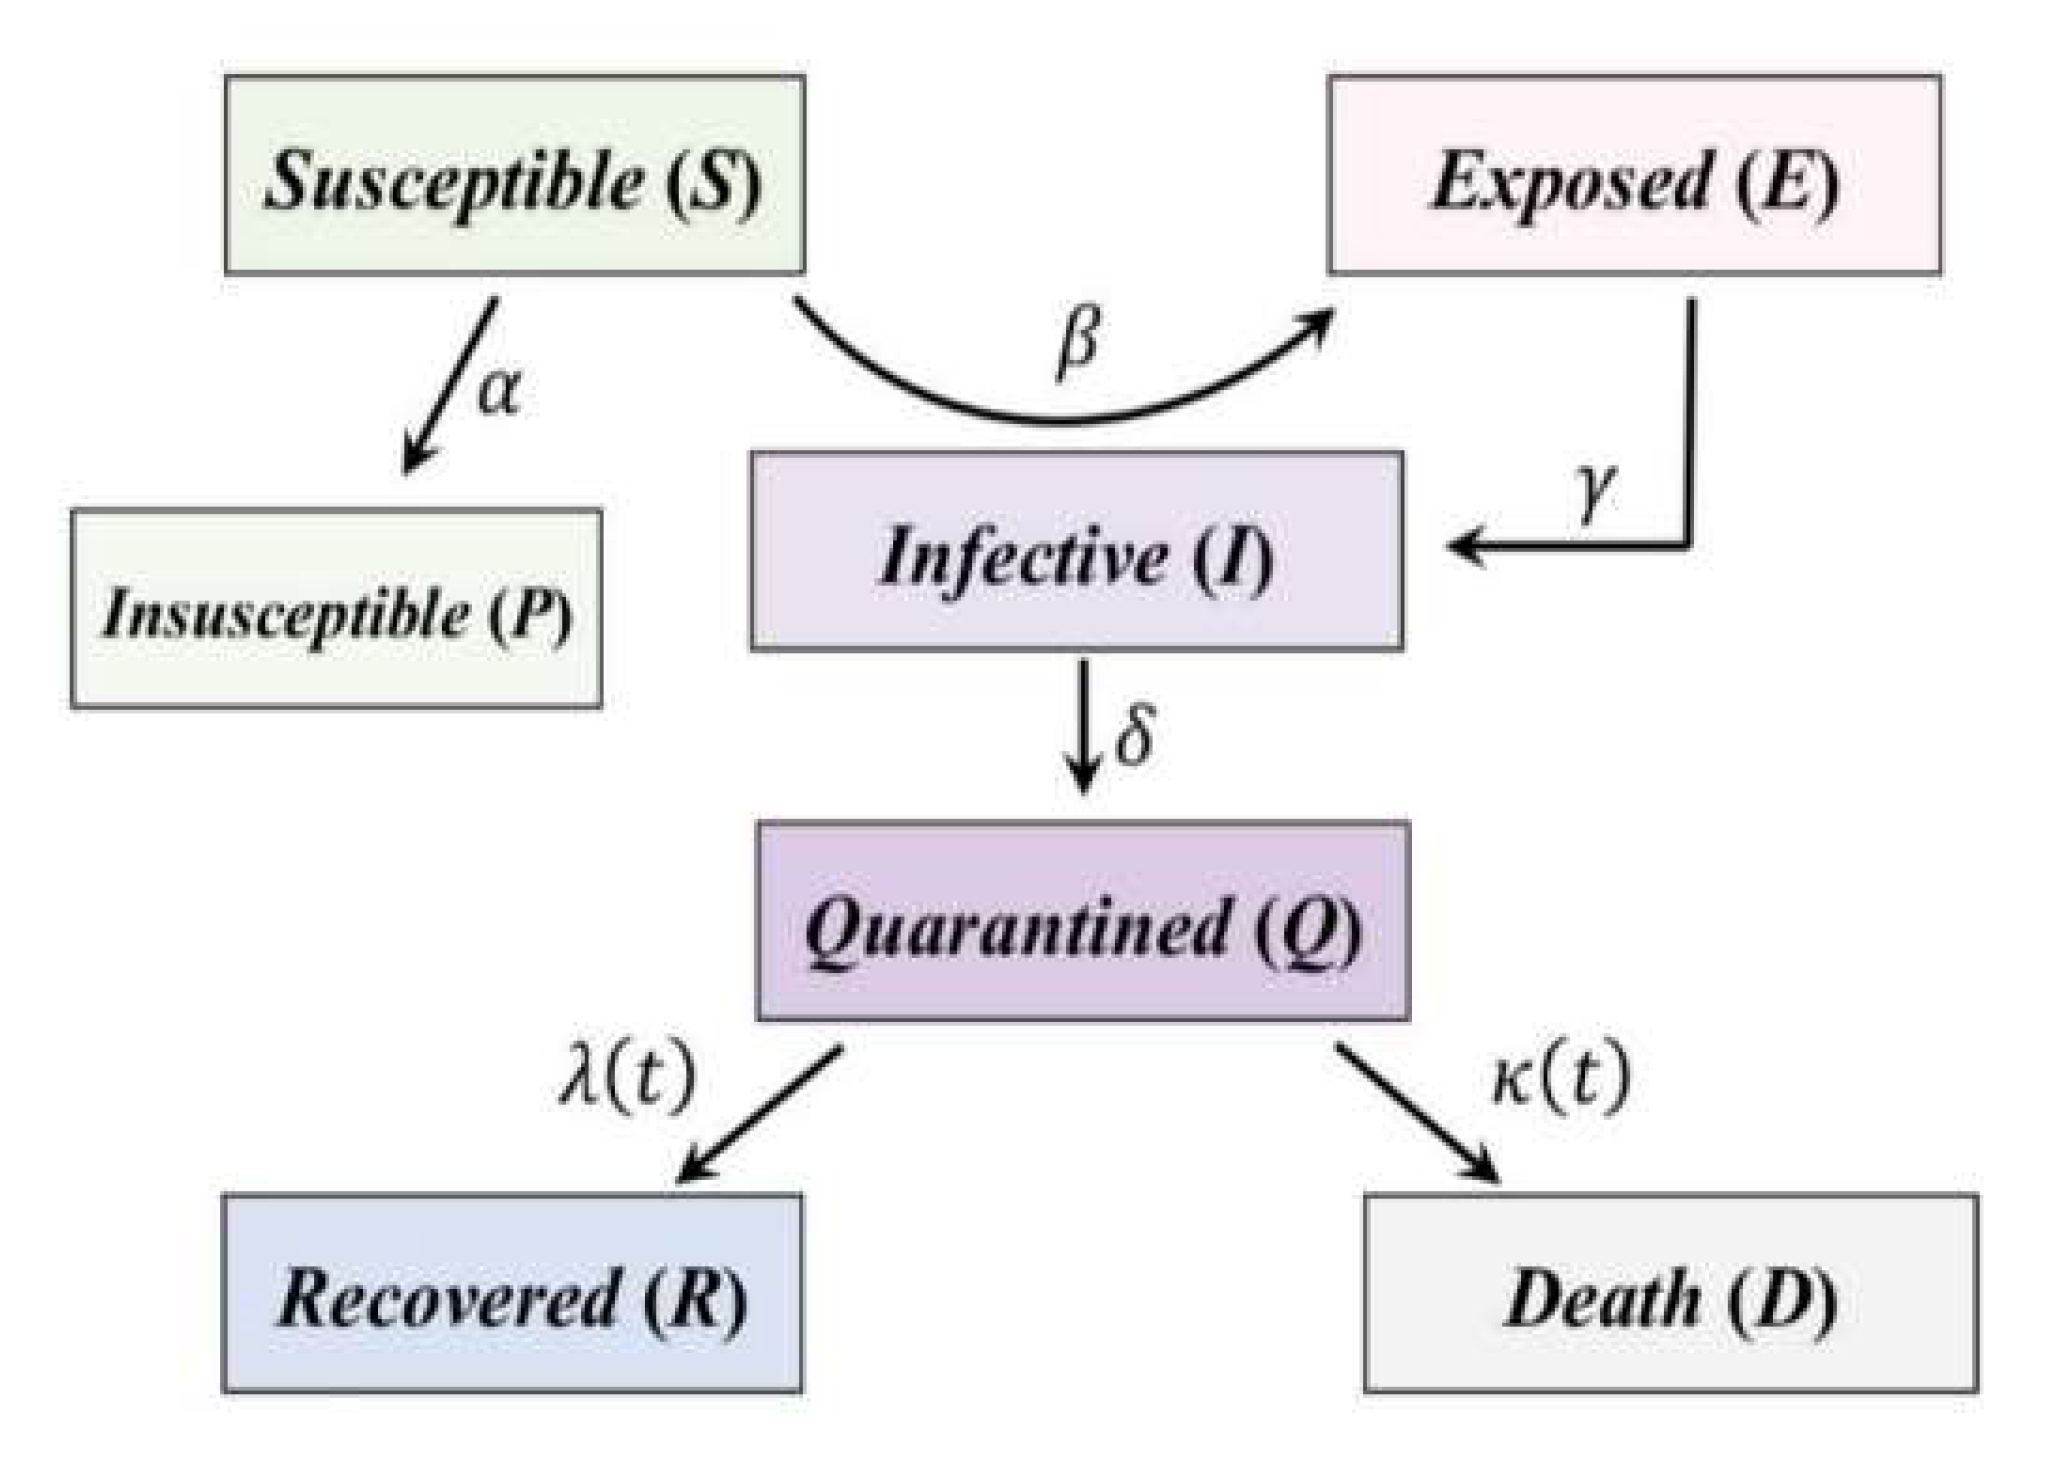
\includegraphics[width=\linewidth]{img/ijerph-17-03535-g001.png}
    \caption{Esempio di modello SEIR preso dall'articolo \cite{ijerph17103535}}
    \label{fig:SEIR_model}
\end{figure}

Il motivo per cui viene utilizzato il modello SEIR come base è perchè permette di 
modellare una caratteristica intrinseca di una malattia infettiva, ovvero 
il periodo di latenza che un individuo appena infettato ha prima di diventare 
infettivo a sua volta e mostrare i sintomi di infezione. Questo permette 
di osservare quanto le misure di sicurezza e prevenzione non farmaceutiche 
sono efficaci sulla popolazione tenendo in considerazione 
un tempo di ritardo intrinseco nel feedback tra l'attuamento delle 
misure di prevensione e i risultati positivi di queste ultime.

Una delle modifiche più utilizzate a questo modello è quella di avere un sistema 
ciclico, ovvero in cui gli individui che entrano nello stato R non diventano immuni 
alla malattia a tempo indefinito, ma perdono questa loro caratteristica di immunità
dopo un dato periodo di tempo. Questo permette di modellare con più accuratezza le malattie
infettive stagionali come ad esempio la comune influenza o il raffreddore, oppure 
mostrare l'andamento ad ondate di altre malattie che hanno la caratteristica di 
mutare molto velocemente, come è stato per il COVID-19 e le sue innumerevoli varianti.

\newpage

\begin{figure}[h]
    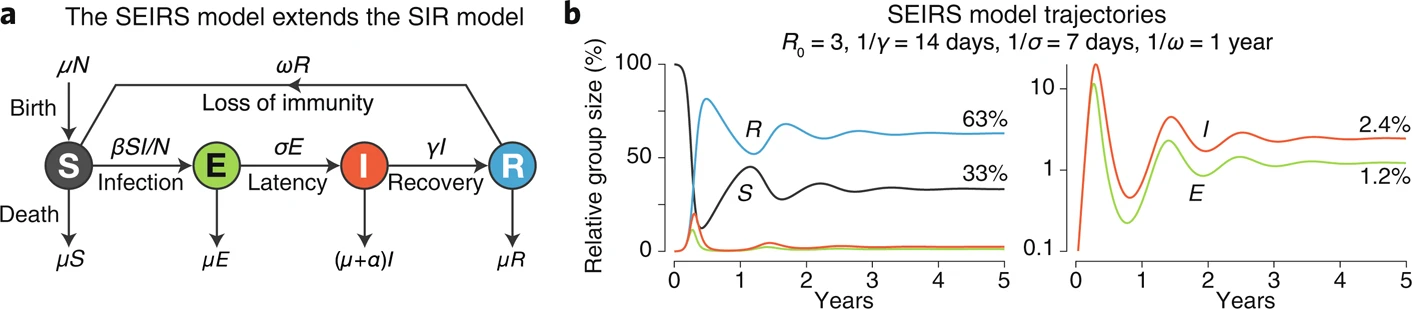
\includegraphics[width=\linewidth]{img/41592_2020_856_Fig1_HTML.png}
    \caption{Modello SEIRS preso dall'articolo \cite{Bjornstad2020}}
    \label{fig:SEIRS_model}
\end{figure}

Questa variante denominata SEIRS permette invece di osservare, non solo l'andamento e 
l'efficacia delle contromisure non farmaceutiche, ma anche di quelle
farmaceutiche, come ad esempio i vaccini; o più in generale l'andamento
della così detta immunità di gregge \cite{Bjornstad2020}. 

Rimanendo sull'idea di voler analizzare l'efficacia di un vaccino, una
modifica comune al modello SEIR è quella legata all'aggiunta dello stato V,
Vaccinated, come stato esplicito oppure oppure implicito al modello. Questa 
variazione permette di modellallare con più attenzione l'efficacia di un 
vaccino una volta introdotto all'interno della popolazione, 
ma più in generale permette di osservare l'efficacia di una politica di vaccinazione 
in relazione al numero di vaccinazioni effettuate in un determinato periodo di tempo.
Questo viene solitamente affiancato con un modello ciclico, così da poter
osservare come bisogna modificare le proprie politiche vaccinali in vista
di ondate cicliche più o meno intense di infezioni.

\begin{figure}[h]
    \begin{center}
        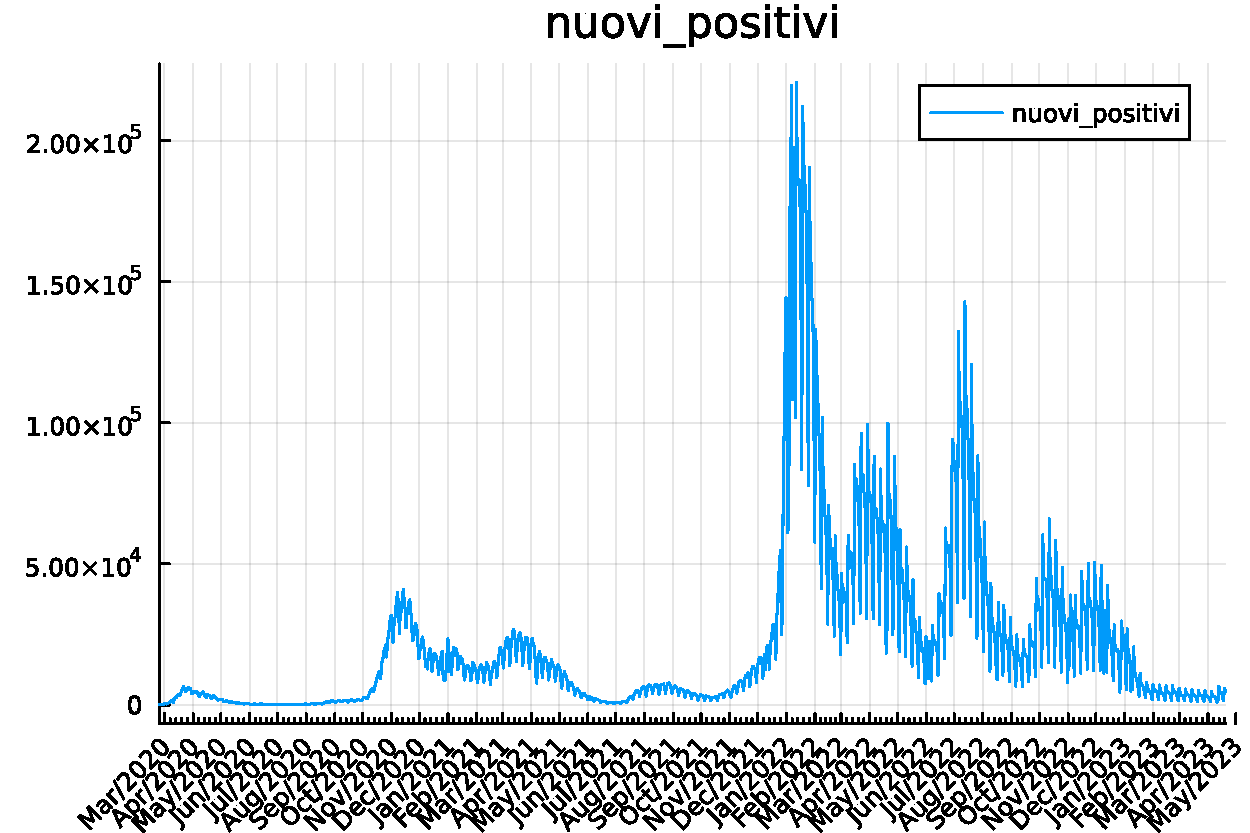
\includegraphics[scale=0.6]{img/nuovi_positivi_2023-04-21.pdf}
        \caption{Esempio di ondate di infettività. Dati del Dipartimento di Protezione Civile Italiana}
        \label{fig:DPC_new_positive}
    \end{center}
\end{figure}

Ai fini pratici di una simulazione avere uno stato esplicitamente definito
oppure ricavabile dalle probabilità di transizione degli altri stati 
è pressocchè indifferente, e potrebbe essere richiesta una diferenziazione
solamente in caso in cui si avrebbe una differenza sostanziale tra lo stato
R e V, ad esempio in termini di protezione dalla malattia, durata immunità etc... .

% \begin{figure}[h]
%     \begin{center}
%         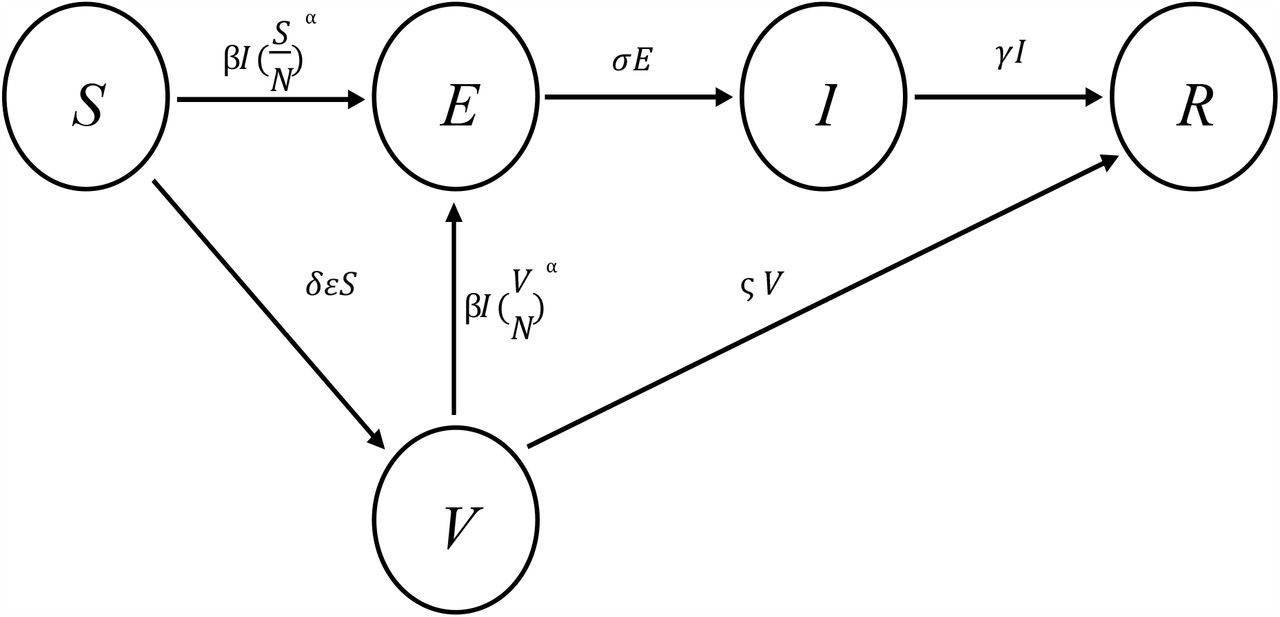
\includegraphics[width=\linewidth]{img/seirv_explicit.jpg}
%         \caption{Esempio di modello SEIRV con stato esplicito per la condizione V}
%         \label{fig:SEIRV_explicit}
%     \end{center}
% \end{figure}

\begin{figure}[h]
    \begin{center}
        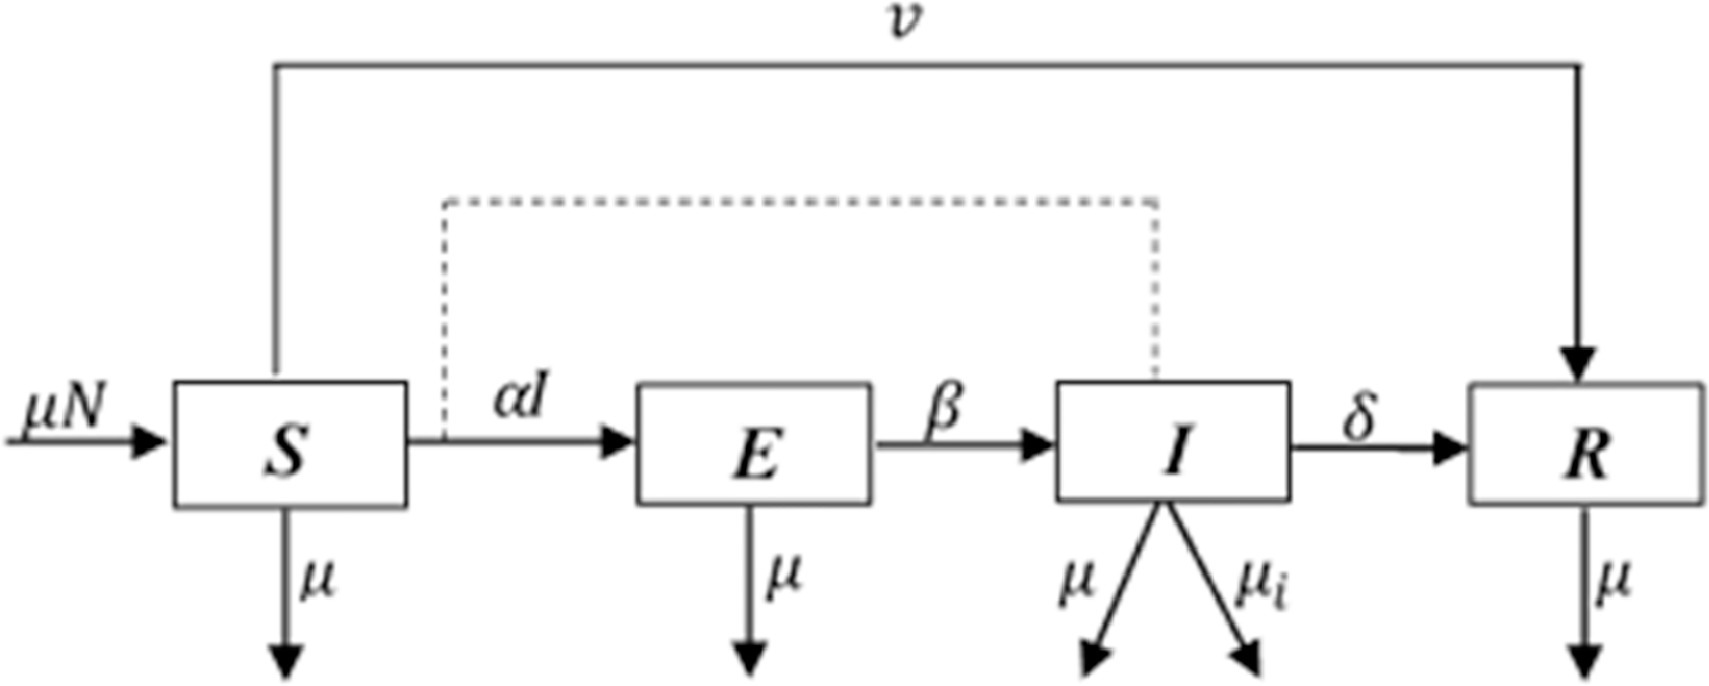
\includegraphics[width=\linewidth]{img/seirv_implicit.jpg}
        \caption{Esempio di modello SEIRV con stato implicito per la condizione V}
        \label{fig:SEIRV_implicito}
    \end{center}
\end{figure}

Non essendoci un numero massimo di stati, e quindi di equazioni, utilizzabili
all'interno del modello, ogni individuo è libero di definire un numero
di equazioni arbitrario che rispecchia la sua idea di modellazione del 
sistema. Ne è un esempio il modello riportato in \cite{Giordano2020}.

Come precedentemente introdotto esistono due grandi famiglie di modelli
per la simulazione, e sono rispettivamente la famiglia di modelli deterministici
e quella di modelli stocastici.

\newpage

\subsubsection{Modelli Deterministici}
I modelli deterministici vengono principalmente utilizzati 
per la loro immediatezza e riproducibilità. Infatti un modello
deterministico, una volta impostati i parametri necessari
riprodurrà sempre lo stesso risultato. Questo tipo di approccio, 
seppur utilizzatto in larga scala come ad esempio da \cite{Bjornstad2020}
\cite{Mwalili2020}, \cite{Giordano2020} si basa su delle assunzioni molto forti
che non sempre rispecchiano la realtà. 

Infatti i modelli deterministici hanno il grosso problema di
essere affidabili solamente nel caso in cui vi siano dati 
sufficientemente grandi, cosa che non sempre è possibile
avere \cite{wiki:Compartmental_models_in_epidemiology}.
Essendo modelli di tipo deterministico, avendo dei parametri 
di infettività maggiori di zero, con un numero di individui infetti
anch'esso maggiore di zero, si tenderà ad avere nel lungo
periodo un andamento di equilibrio endemico derivato 
dalle equazioni e dal modello utilizzato. Questo comportamento
però non sempre rispetta la realtà, ma come precedentemente 
accennato, in casi in cui si hanno grandi quantità di dati 
legati principalmente alla popolazione, questi modelli si 
comportano in maniera affidabile.

\begin{figure}[h]
    \begin{center}
        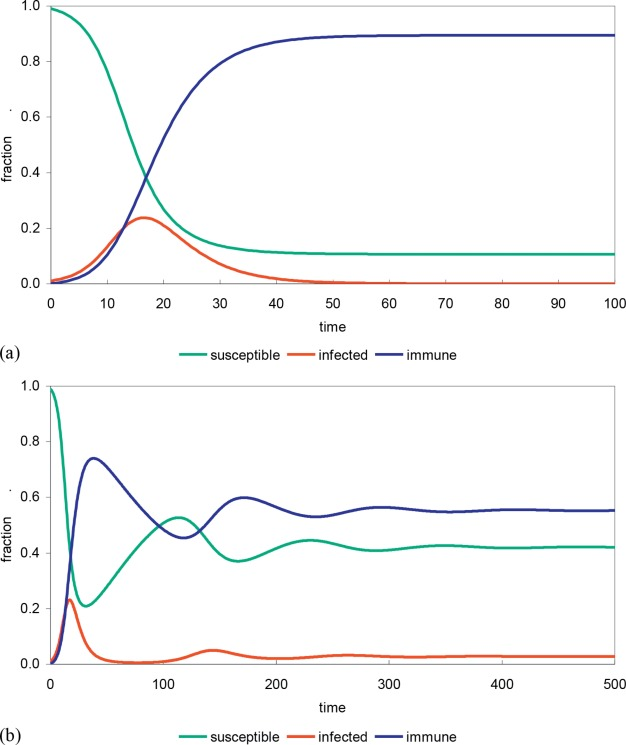
\includegraphics[scale=0.7]{img/3-s2.0-B9780128012383988378-f98837-02-9780128012383.jpg}
        \caption{Esempio equilibrio endemico}
        \label{fig:Endemic_equilibrium}
    \end{center}
\end{figure}

\subsubsection{Modelli Stocastici}
I modelli stocastici, seppur più complessi e non determinabili 
a priori, permettono una modellazione più veritiera e 
simile alla realtà in quanto tengono in considerazione 
variazioni randomiche che possono capitare durante il 
decorso di una pandemia. Tuttavia questa loro caoticità 
richiede che per ottenere risultati robusti debbano essere 
eseguiti e computati molteplici volte, e la media dei loro 
risultati è il valore vero da tenere in considerazione. 
Questi modelli sono stati applicati durante la pandemia da COVID-19 
come ad esempio da \cite{ijerph17103535}. 

\begin{figure}[h]
    \begin{center}
        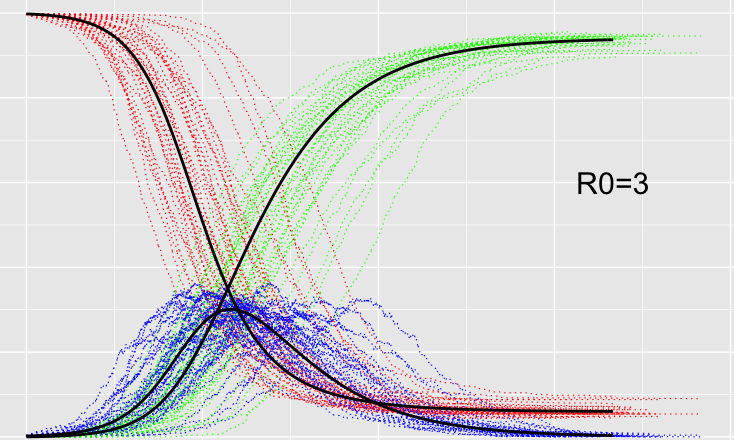
\includegraphics[width=\linewidth]{img/Gillespie-e1643395123662.png}
        \caption{Modello SIR stocastico}
        \label{fig:Endemic_equilibrium_stochastic_sir}
    \end{center}
\end{figure}

E' immediato notare come il comportamento delle curve sia 
imprevedibile se preso singolarmente, e che non sempre 
esiste uno stato di equilibrio endemico chiaro e definito come
quello ottenibile da un modello deterministico. Ciò nonostante 
effettuando molte simulazioni è possibile vedere come il 
comportamento generale del modello sia comunque simile a 
quello di un modello deterministico.